\documentclass[journal]{IEEEtran}
%\documentclass[12pt,journal,draftclsnofoot,onecolumn]{IEEEtran}
%\documentclass[conference]{IEEEtran}

\IEEEoverridecommandlockouts

\usepackage{etex}

%Fixing IEEEtran.cls bug with [english]{babel}
\makeatletter
\def\markboth#1#2{\def\leftmark{\@IEEEcompsoconly{\sffamily}\MakeUppercase{\protect#1}}%
\def\rightmark{\@IEEEcompsoconly{\sffamily}\MakeUppercase{\protect#2}}}
\makeatother

% \usepackage{t1enc}

\usepackage{listings}

%\usepackage[utf8x]{inputenc}
\usepackage[english]{babel}
\selectlanguage{english}
\usepackage{color}
\usepackage{lipsum}% http://ctan.org/pkg/lipsum
%\usepackage{caption}
\usepackage{cite}
\usepackage[pdftex]{graphicx}
%\usepackage{subfig}
%\usepackage{subcaption}
\usepackage{amsmath}
\usepackage{mathtools}
\usepackage{amsfonts}
\usepackage{array}
\usepackage{verbatim}
\usepackage{listings}
\usepackage{hyperref}
\usepackage{url}
\usepackage{enumerate}
\usepackage{multirow}

\usepackage{epsfig}
\usepackage{epstopdf}
\usepackage{multicol}% http://ctan.org/pkg/multicols
\usepackage[font=footnotesize]{caption}
\usepackage[font=scriptsize]{subcaption}
% Tikz
\usepackage{tikz}
\usepackage{pgfplots}
\pgfplotsset{compat=newest}
\pgfplotsset{plot coordinates/math parser=false}
\newlength\fheight
\newlength\fwidth
\usetikzlibrary{patterns,decorations.pathreplacing,backgrounds,calc}
\definecolor{SchoolColor}{RGB}{0.71, 0, 0.106}%181,0,27} unipd red
\definecolor{chaptergrey}{rgb}{0.61, 0, 0.09} % dialed back a little
\definecolor{midgrey}{rgb}{0.4, 0.4, 0.4}
\definecolor{chaptergreen}{rgb}{0.09, 0.612, 0}
\definecolor{chapterpurple}{rgb}{0.522, 0, 0.612}
\definecolor{chapterlightgreen}{rgb}{0, 0.612, 0.522}

%\raggedbottom

% Pseudocode
\usepackage[ruled, vlined]{algorithm2e}
\SetKwRepeat{Do}{do}{while}
\SetKwBlock{wpPa}{with probability $P_A$}{end}
\DontPrintSemicolon
% \usepackage{algorithm}
% \usepackage[noend]{algpseudocode}
% \renewcommand\algorithmicthen{}
% \renewcommand\algorithmicdo{}
\usepackage{lscape}
\usepackage{setspace}

\addto\captionsenglish{\renewcommand{\figurename}{Fig.}}

\newcommand{\field}[1]{\mathbb{#1}}

\DeclareMathOperator*{\argmin}{arg\,min}
\DeclareMathOperator*{\argmax}{arg\,max}
\newcommand{\norm}[1]{\left\lVert#1\right\rVert}
\renewcommand{\arraystretch}{2}

\newcommand{\DP}[1]{\textbf{(DP: #1)}}
\newcommand{\el}[1]{\textr{(EL says: #1)}}
\newcommand{\fm}[1]{\texbf{(FM says: #1)}}

\usepackage{threeparttable}
%\usepackage[table,xcdraw]{xcolor}
\usepackage{tabularx}
\usepackage{multirow}
\usepackage{booktabs}
\newcommand{\tabitem}{~~\llap{\textbullet}~~}
\usepackage{array, blindtext}
\usepackage{wrapfig}
\usepackage{pdfpages}
\usepackage[acronym]{glossaries}

% use tikArchiviz images or eps
\newif\iftikz
\tikztrue

\graphicspath{{./figures/}}

\title{Heuristic optimization of Distributed Storage Network techniques}
\author{\IEEEauthorblockN{Federico Mason$^*$, Davide Peron$^*$, Enrico Lovisotto$^*$}\\
\small{{$^*$Department of Information Engineering, University of Padova -- Via Gradenigo, 6/b, 35131 Padova, Italy\\
Email: {\tt\{masonfed,perondav,lovisott\}@dei.unipd.it}\\}}
}

% Reduce the space below figs.
%\setlength{\belowcaptionskip}{-0.7cm}

%% Glossary
\newacronym{dsn}{DSN}{Distributed Storage Network}
\newacronym{edfc}{EDFC}{Exact Decentralized Fountain Codes}
\newacronym{adfc}{ADFC}{Approximate Decentralized Fountain Codes}
\newacronym{sa}{SA}{Simulated Annealing}
\newacronym{ga}{GA}{Genetic Algorithm}
\newacronym{jb}{JB}{Jumping Ball}
\newacronym{wsn}{WSN}{Wireless Sensor Network}
\newacronym{fp}{FP}{First Problem}
\newacronym{sp}{SP}{Second Problem}
\newacronym{of}{$f$}{Objective Function}
\newacronym{t}{T}{Temperature}
\newacronym{oc}{$x_o$}{Old Candidate}
\newacronym{nc}{$x_n$}{New Candidate}
\newacronym{sc}{$C_S$}{Step Coefficient}
\newacronym{ac}{$C_A$}{Acceptance Coefficient}
\newacronym{ap}{$P_A$}{Acceptance Probability}
\newacronym{ws}{$N_{WS}$}{Number of Worsening Steps}
\newacronym{wsmax}{$N_{WS}^{MAX}$}{ Maxiumum Number of Worsening Steps}
\newacronym{x}{x}{Candidate}
\newacronym{bestx}{$x_{best}$}{Best candidate}

\glsresetall
\begin{document}

\setlength{\belowcaptionskip}{-0.2cm}

% reduce space after title
\makeatletter
\patchcmd{\@maketitle}
  {\addvspace{0.5\baselineskip}\egroup}
  {\addvspace{-1.2\baselineskip}\egroup}
  {}
  {}
\makeatother

\maketitle

\begin{abstract}
In some previous works about \gls{dsn}, two packet spreading algorithm are presented, \gls{edfc} and \gls{adfc}.

Unfortunately the tuning of their fundamental parameters, $x_d$ and $\nu(d)$ respectively, was not thoroughly investigated.

We try to perform such tuning applying some heuristic optimization techniques, such as \emph{Simulated Annealing} and \emph{Genetic Algorithm}, in order to explore the solution space of the problem.

\end{abstract}

\begin{IEEEkeywords}
Distributed Storage Networks, sensors, heuristic optimization
\end{IEEEkeywords}

\glsresetall
\label{sec:introduction}
We consider a \gls{wsn} whose nodes are distributed over a known region.
Some of them, called \textit{sensing nodes}, collect and deploy data from the environment (temperature, pressure, motion data, \ldots) while the others, called \textit{caching nodes}, simply store data coming from \textit{sensing nodes}.

In literature, a \gls{wsn} often has a central node, a powered sink connected to the internet.
Such special node receives all information collected by the nodes in the network and provides it to the users.

However, in our paper, following what has been done in \cite{Lin2007}, we get rid of this assumption.
Users then must collect the data stored in the network visiting the geographical region where system is located.

In such a scenario, user visits only a certain number $h$ of nodes of the network.
Our reference paper \cite{Lin2007}, guarantees source packets decodability using \emph{Random Fountain Codes}, combining and spreading $K$ source packets across $N$ total nodes such that, using any group of $K+\epsilon$ of them (with $\epsilon$ constant in $K$), the original information can be successfully retrieved with high probability.

The challenge here is to keep the communication cost at a minimum level, while keeping the failure probability low.

Traditional but expensive two-way packet delivery is then discarded, in favour of one-way \emph{random walks}.
Random walks are designed according to \emph{Metropolis algorithm} such that the number of packets reaching each node resembles the Robust Soliton distribution, whose optimal decoding properties are known\cite{Luby}.

In this paper, we are going to find the optimal $x_d$ and $\nu(d)$ parameters for \gls{edfc} and \gls{adfc} respectively, with three different heuristics.

The optimal configurations are then tested with a network simulator, where further analysis is performed.

The article is structured in three sections.

In \autoref{sec:tech_approach} we present in detail the heuristic algorithms employed, first with a general description of the framework and then fucusing on our specific problem.

In \autoref{sec:results} we present the results obtained using the optimal parameter configurations in the network simulator we have implemented.

\section{Technical Approach}
\label{sec:tech_approach}

\gls{edfc} and \gls{adfc} spreading algorithms require to be tuned, with their parameters $x_d$ and $\nu(d)$.

$x_d$ is a K-dimensional variable of \gls{edfc} called \textit{redundancy coefficent}. Given a node with \textit{code degree} $d$, $x_d \cdot d$ represents the number of packets that should be received by the node itself at the end of packets spread.

The best value of $x_d$ is the solution of the following optimization problem\cite{Lin2007}.

\begin{equation}
	\label{firstproblem}
	\begin{split}
		minimize & \sum_{d=1}^K x_d d \mu (d) \\
		subject \ to & \begin{dcases}
			Pr(Y<d|X=d) \leq \delta_d \\
			x_d \geq 1 \quad for \quad d = 1,...,K
		\end{dcases}
	\end{split}
\end{equation}

$\nu$ is instead the degree distribution of network nodes such that, after package spread, the resulting degree distribution $\nu^\prime$ is as close as possible to the \textit{Robust Soliton Distribution}.

The optimal $\nu(d)$ is the solution of the following optimization problem\cite{Lin2007}.

\begin{equation}
	\label{secondproblem}
	\begin{split}
		minimize & \quad \sum_{i=1}^{K/R}(\nu'(i)-\mu(i))^2 \\
		subject \ to & \quad \begin{cases}
			\sum_{i=1}^K \nu(i) = 1 \\
			\nu(i) \geq 0 \quad for \quad i=1,...,K
		\end{cases}
	\end{split}
\end{equation}

given
\begin{equation*}
	\begin{split}
		& v^\prime(i) = \sum_{d=1}^K \nu(d) \binom{K}{i} p(d)^i [1-p(d)]^{K-i} \\
		& p(d) = 1 - \left(1 -\frac{d}{N E}\right)^{\frac{N E}{K}} \\
		& E = \text{ expected value of }\nu
	\end{split}
\end{equation*}

From now on, we call \eqref{firstproblem} and \eqref{secondproblem} simply \gls{fp} and \gls{sp}.

We see immediately that \gls{fp} and \gls{sp} are not solvable with \emph{convex optimization} tecniques, as they don't minimize convex objective functions over convex sets.

To overcome this issue, we chose the heuristic approach, whose convergence to the optimum is not guaranteed in polynomial time, but whose effectiveness has been proven in many fields \cite{Edelkamp2010} where traditional tools (such as \emph{Simplex}) cannot be applied.

In fact they reach solutions that are often suboptimal but still useful for our purposes.

\subsection{Simulated Annealing}

The first algorithm we implement is known as \gls{sa}.
\gls{sa} is a probabilistic technique that takes ispiration from annealing in metallurgy, a process that aims to reduce materials defects.
In this physical process a piece of metal is warmed at high temperatures and then slowly cooled. In this way it is possible to achieve the molecular equilibrium inside the material itself.

In \gls{sa}, we treat \gls{of} as the internal energy of the material.
As in the physical process we want to reduce the function energy and the slowly bring it to a stable value. In other words we want first cross widely the function domain and then concentrate in the points with higher probability to be the absolute minimum of \gls{of}.

\gls{sa} behaviour is dependent on a parameter called \gls{t}: relevant for the search are \gls{sc} and \gls{ac}, the number of points to inspect for given \gls{t} and the probability $P_A$ of accepting a point worse than the current, respectively.

At the beginning \gls{t} is initialized at a sufficient high value and then it is reduced at each algorithm step.

The process starts at a random point that respect problem constraints. Each new point $\vec{x}_{new}$ is found \emph{perturbing} previous vector $\vec{x}$ until one is found that respects problem constraints.
Such solution is kept or rejected according to the \gls{ap}, whose expression is the following.

 \begin{equation*} \label{accept_prob}
	P_A(T) = \begin{cases}
		1 & f(\vec{x}_n)-f (\vec{x}_o) < 0 \\
		\exp{ \left( C_A(T) \frac{
					\, [f(\vec{x}_n) - f(\vec{x}_o)] }{T} \right) }
		& f (\vec{x}_n)-f(\vec{x}_o) \geq 0
  \end{cases}
 \end{equation*}

Empirically, we found that a successful perturbation strategy for this problem is adding an uniform variable, whose range is proportional to temperature, to a randomly chosen component of the $\vec{x}$ vector.

The best point among all the explored ones is kept at each iteration and it is returned at the end of the computation.

The algorithm is provided here as pseudocode.

\begin{algorithm}
\KwIn{Objective function $f$ and constraints, Initial Temperature,  Steps Coefficient, Acceptance Coefficient}
\KwOut{Optimal solution}
\caption{Simulated Annealing}
$T \gets$ Initial Temperature \\
$x \gets$ Candidate \\
$x_{best} \gets x$ \\
$C_S \gets$ Step coefficient \\
$C_A \gets$ Acceptance coefficient \\

\While{$T>0$}{
	\For{$i = 1$ to $SC$}{
		\vspace{1mm}
		$x_0 \gets x$\\
		$x_n \gets Neighbour(x)$\\
		\While{$x_n$ doesn't respect costraints} {
			$x_n \gets Neighbour(x)$\\
		}
		$P_A \gets$ Acceptance probability \\
		\wpPa {
			\vspace{1mm}
			$x \gets x_n$\\
		}
	}
	update $T$\\
	update $C_S(T)$\\
	uptade $P_A(C_A)$\\
	\If{$f(x)<f(x_{best})$}{
		\vspace{1mm}
			$x_{best} \gets x$\\
		}
	}
	\Return{$x_{best}$}
\end{algorithm} % \captionof{lstlisting}{Simulated Alleaning} \label{code_sa}

\subsection{Jumping Ball}

The second technique we implent is called \gls{jb}. \gls{jb} is a variant of \gls{sa} and apparently it follows the same operating model. The difference between \gls{jb} and \gls{sa} is that the searching for the best \gls{x} could make a \textit{jump}. This means that in some circumstances the value of \gls{nc} is not choosen between the neighbours of \gls{x} but between points rather distant from \gls{x}. These \textit{jumps} make the search  varies along the \gls{of} domain widely than what happens in \gls{sa}.

Let's compare pseudocode of \gls{sa} with pseudocode of \gls{jb}. We note immediately that they have almost the same pattern. As \gls{sa}, \gls{jb} is based on the parameter \gls{t}. Every time that \gls{t} decreases a new step of the algorithm begins. At every new step \gls{jb} uptades the values of \gls{sc}, \gls{ac} and consequently \gls{ap}. As in \gls{sa} the values of these parameters determine how the algorithm moves through the function domain searching for a new \gls{nc}.

Looking more carefully at pseudocode of \gls{jb}, we note that this algorithm uses two parameters that \gls{sa} doesn't. These parameters are called \gls{ws} and \gls{wsmax}. During the \textit{inizialization phase}  \gls{ws} and \gls{wsmax} are respectively set to zero and to a positive value. While \gls{wsmax} is fixed, \gls{ws} changes value as the algorithm goes on. To understand the working of \gls{ws} and \gls{wsmax} we suppone that \gls{jb} moves to \gls{nc}. If \gls{nc} has better performance than \gls{oc} ($P_A=1$) the value of \gls{ws} is immediately set to zero again. Instead if \gls{nc} has worse performance than \gls{oc} ($P_A<1$) the value of \gls{ws} is increased of one. We conclude that \gls{ws} increases as the algorithm moves to points with worse performance than the points already crossed.

Putting ourself in a very unlucky scenario we suppone that for several times consecutively the new value of \gls{x} is worse than the previous one. In this case the value of \gls{ws} increases al lot, untill it becomes close to \gls{wsmax}. When \gls{ws} exceeds \gls{wsmax} the \textit{jump} takes place. This mean that for a single time the searching for \gls{nc} change its working. In particular the perturbation which \gls{x} is subjected is much bigger. In addiction to have more intensity the perturbation doesn't envolve only one component of \gls{x} but a random number of them. Then \gls{nc} is not a neighbour of \gls{x} anymore but is a point very far from it in the functon domain. After the \textit{jump} the value of \gls{ws} is set to zero and the algorithm goes on as nothing happens. In a simply way we can say that at evry \textit{jump} the algorithm changes the starting point of its searching.

We note that in \gls{jb} is fundamental inizialize accurately the value of \gls{wsmax}. If we choose a value to low, the algorithm will make a huge series of consecutives jump without ever stabilizing in a single area. Conversely if we choose a value too high, the algorithm will never find itself in a condition in which it has to \textit{jump}. We can admit that if we let \gls{wsmax} goes to infinity, \gls{jb} becomes identical to \gls{sa}.

In \gls{sa} we risk that the algorithm focus the search in a bad area, without being able to improve the solution already found. In \gls{jb} this unlucky case is always avoid thanks to \textit{jumps}.


\pagebreak
\begin{algorithm}
	\KwIn{Objective function and constraints, \textit{survival rate}, \textit{max generations}, $\norm{population}$}
	\KwOut{Optimal solution}
	$T \gets Temperature$\\
	$x \gets Candidate$\\
	$x_{best} \gets x$\\
	$C_S(T) \gets \textit{Step coefficient}$\\
	$C_A(T) \gets \textit{Acceptance coefficient}$\\
	$P_A(C_A) \gets \textit{Acceptance probability}$\\
	$N_{WS} \gets 0$\\
	\While{$T>0$}{
		\For{$i = 1$ to $SC$}{
			$x_0 \gets x$\\
			$x_n \gets Neighbour(x)$\\
			\While{$x_n$ doesn't respect costraints}{
				\textit{$N_{WS}++$}\\
				\If{$N_{WS}<N_{WS}^{MAX}$}{
					$x_n \gets Neighbour(x)$\\
				}
				\Else{
					$x_n \gets Jump(x)$\\
					$N_{WS} \gets 0$
				}
			}
			\wpPa{
				$x \gets x_n$\\
			}
		}
		update $T$\\
		update $C_S(T)$\\
		update $C_A(T)$\\
		uptade $P_A(C_A)$\\
		\If{$F_O(x)<F_O(x_{best})$}{
			$x_{best} \gets x$\\
		}
	}
	\Return{$x_{best}$}
	\caption{Jumping Ball}\label{algo:JB}
\end{algorithm}

\subsection{Genetic Algorithm}
The third technique is called Genetic Algorithm.
The algorithm takes randomly an initial set of solution for the problem, called \textit{population}, and tries to evolve it toward better solutions.
Each candidate solution is called \textit{individual}, that is usually a multi-dimensional array. In biological applications, each component of the individual is a \textit{chromosome} or a \textit{genotype}, in our case it is simply an entry for the array.

\gls{ga} is an iterative process, in each iteration, the population is evolved in a new \textit{generation}.
In each generation, the objective function of each individual is evaluated. The best individuals (in terms of objective function) are selected and mutated to create the next generation.

The way in which an individual is mutated can be arbitrarily chosen.
Usually one or more components are perturbated randomly, or parts of different solutions are joined togheter, to maintain the properties of the old solutions trying to improve it.
In this work we have decided to perturbe each individual up to 3 times, the number of perturbation will be the one that leads to a better objective function.

\begin{algorithm}
\KwIn{Objective function and constraints, \textit{survival rate}, \textit{max generations}, $\norm{population}$}
\KwOut{Optimal solution}
$generation \gets 0$\\
$\textit{best part size} \gets \norm{population} \cdot \textit{survival rate}$\\
$population \gets \textit{initial population}$\\
\While{$generation < \textit{max generations}$}{
  sort(\textit{population})\\
  \For{$j=1$ to round($1/\textit{survival rate}$)}{
    \For{$i=1$ to \textit{best part size}}{
      $population(j \cdot \textit{best part size} + i) \gets population(i)$\\
      \Do{! respect Constraints}{
        $individual \gets population(j \cdot \textit{best part size} + i)$\\
        $candidates(0) \gets individual + perturbation$\\
        $candidates(1) \gets candidate(0) + perturbation$\\
        $candidates(2) \gets candidate(1) + perturbation$\\
        sort(\textit{candidates})\\
        $individual \gets candidates(0)$
      }
      $population(j \cdot \textit{best part size} + i) \gets individual$
    }
  }
  \textit{generation++}
}
\Return{$population(0)$}\;
\caption{Genetic Algorithm}\label{algo:GA}
\end{algorithm}

The parameters that can be tuned in order to achieve the best result are:
\begin{description}
	\item[\textbf{Survival Rate}] \hfill \\
	The fraction of population that is used to create the next generation;
	\item[\textbf{Max Generations}] \hfill \\
	Number of generations created, this is actually the number of iteration of the algorithm. The duration of the computation is linearly dependent on this parameter.
	\item[$\norm{population}$] \hfill \\
	Number of individual in a population. This parameter affects the computational complexity of the algorithm. The larger the population, the more time will pass from one generation to another, since in each generation the objective function for each individual is computed.
\end{description}

\section{Results}
\label{sec:results}
\begin{figure}
  \centering
	    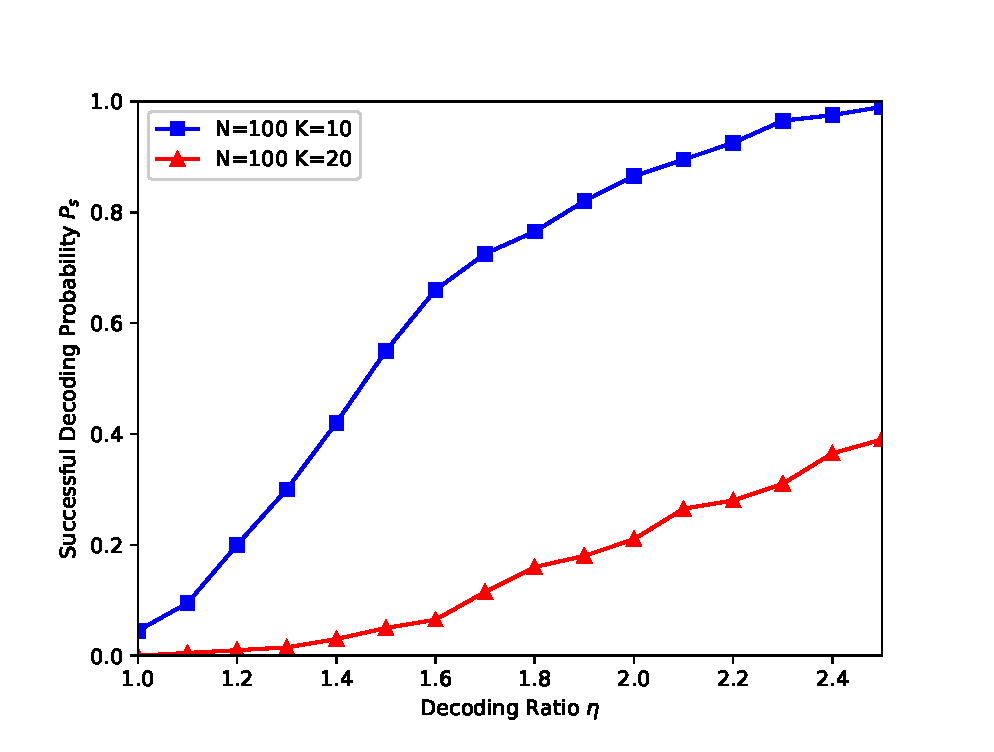
\includegraphics[width=0.9\columnwidth]{ratiovsprob.eps}
  \caption{Successfull decoding probability $P_s$ for different values of $N$, $K$ and decoding ratio $\nu$.}
  \label{fig:ratiovsprob}
\end{figure}

\section{Conclusions And Future Work}
\label{sec:conclusions}

\bibliographystyle{IEEEtran}
\bibliography{bibliography}

\end{document}
